\documentclass{beamer}
\usepackage[T1]{fontenc}
\usepackage[utf8]{inputenc}

\usetheme{Madrid}
\usecolortheme{default}
\usepackage{amsmath,amssymb,amsfonts,amsthm}
\usepackage{txfonts}
\usepackage{tkz-euclide}
\usepackage{listings}
\usepackage{adjustbox}
\usepackage{array}
\usepackage{tabularx}
\usepackage{gvv}
\usepackage{lmodern}
\usepackage{gensymb}
\usepackage{circuitikz}
\usepackage{tikz}
\usepackage{graphicx}
\usepackage{capt-of}

\setbeamertemplate{page number in head/foot}[totalframenumber]

\usepackage{tcolorbox}
\tcbuselibrary{minted,breakable,xparse,skins}

\definecolor{bg}{gray}{0.95}
\DeclareTCBListing{mintedbox}{O{}m!O{}}{%
  breakable=true,
  listing engine=minted,
  listing only,
  minted language=#2,
  minted style=default,
  minted options={%
    linenos,
    gobble=0,
    breaklines=true,
    breakafter=,,
    fontsize=\small,
    numbersep=8pt,
    #1},
  boxsep=0pt,
  left skip=0pt,
  right skip=0pt,
  left=25pt,
  right=0pt,
  top=3pt,
  bottom=3pt,
  arc=5pt,
  leftrule=0pt,
  rightrule=0pt,
  bottomrule=2pt,
  toprule=2pt,
  colback=bg,
  colframe=orange!70,
  enhanced,
  overlay={%
    \begin{tcbclipinterior}
    \fill[orange!20!white] (frame.south west) rectangle ([xshift=20pt]frame.north west);
    \end{tcbclipinterior}},
  #3,
}
\lstset{
    language=C,
    basicstyle=\ttfamily\small,
    keywordstyle=\color{blue},
    stringstyle=\color{orange},
    commentstyle=\color{green!60!black},
    numbers=left,
    numberstyle=\tiny\color{gray},
    breaklines=true,
    showstringspaces=false,
}

\title{4.10.10}
\subtitle{Distance between 2 points}
\author{EE25BTECH11010 - Arsh Dhoke}
\date{}
\begin{document}


\begin{frame}
  \titlepage
\end{frame}

\begin{frame}{Question}
Find the distance of the point $(-1,-5,-10)$ from the point of intersection of the line $\vec{r} = 2\vec{i} - \vec{j} - 2\vec{k} + \lambda (3\vec{i} + 4\vec{j} + 2\vec{k})$ and the plane $\vec{r}\cdot(\vec{i}-\vec{j}+\vec{k}) = 5$.

\end{frame}

\begin{frame}{Input parameters}
\begin{tabular}{|c|c|}
\hline
\textbf{Name} & \textbf{Value} \\ \hline
$\vec{A}$ & $\myvec{2 & 1 \\0 & 3}$ \\ \hline
\end{tabular}

\end{frame}

\begin{frame}{Intersection}
At intersection: 
\begin{align}
\vec{n}^T(\vec{a} + \lambda \vec{b}) = c
\end{align}
\begin{align}
\lambda = \frac{c - \vec{n}^T \vec{a}}{\vec{n}^T \vec{b}}
\end{align}
\begin{align}
\vec{x} = \vec{a} + \left(\frac{c-\vec{n}^T\vec{a}}{\vec{n}^T\vec{b}}\right)\vec{b}
\end{align}
\end{frame}

\begin{frame}{Computation}
\begin{align}
\vec{n}^T \vec{a} = \myvec{1 & -1 & 1}\myvec{2 \\ -1 \\ -2} = 1
\end{align}
\begin{align}
\vec{n}^T \vec{b} = \myvec{1 & -1 & 1}\myvec{3 \\ 4 \\ 2} = 1
\end{align}
\begin{align}
\vec{x} = \myvec{2 \\ -1 \\ -2} + \frac{(5-1)}{1}\myvec{3 \\ 4 \\ 2}
= \myvec{14 \\ 15 \\ 6}
\end{align}
\end{frame}

\begin{frame}{Distance}
\begin{align}
\norm{\vec{P}-\vec{x}} = \sqrt{(14 - (-1))^2 + (15 - (-5))^2 + (6 - (-10))^2}
\end{align}
\begin{align}
= \sqrt{15^2 + 20^2 + 16^2}
= \sqrt{881}
\end{align}
\end{frame}

\begin{frame}{Graph}
\centering
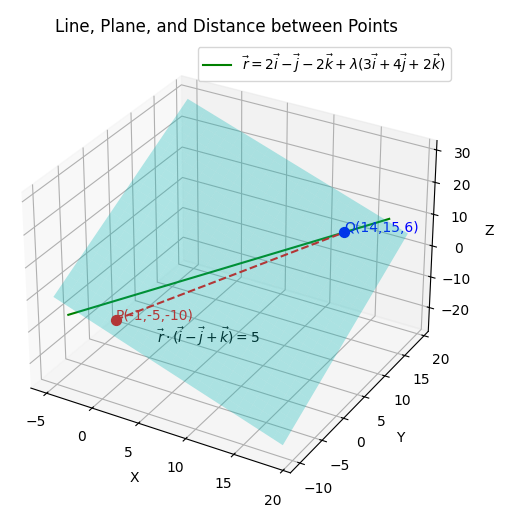
\includegraphics[height=0.7\textheight]{figs/q8.png}
\end{frame}


\begin{frame}[fragile]
    \frametitle{C Code}
\begin{lstlisting}
#include <math.h>

double point_line_plane_distance(
    double Px, double Py, double Pz,
    double ax, double ay, double az,
    double bx, double by, double bz,
    double nx, double ny, double nz,
    double c
) {
    double dot_na = nx*ax + ny*ay + nz*az;
    double dot_nb = nx*bx + ny*by + nz*bz;

    double lambda = (c - dot_na) / dot_nb;

    double Xx = ax + lambda * bx;
    double Xy = ay + lambda * by;
    double Xz = az + lambda * bz;
\end{lstlisting}
\end{frame}

\begin{frame}[fragile]
    \frametitle{C Code}
\begin{lstlisting}
    double dx = Px - Xx;
    double dy = Py - Xy;
    double dz = Pz - Xz;

    return sqrt(dx*dx + dy*dy + dz*dz);
}

\end{lstlisting}
\end{frame}

\begin{frame}[fragile]
    \frametitle{Python Code}
\begin{lstlisting}
import numpy as np
import matplotlib.pyplot as plt
from mpl_toolkits.mplot3d import Axes3D

# Given data
a = np.array([2, -1, -2])      # point on line
b = np.array([3, 4, 2])        # direction vector of line
n = np.array([1, -1, 1])       # normal vector of plane
P = np.array([-1, -5, -10])    # external point

# Intersection point with plane
lam = (5 - np.dot(n, a)) / np.dot(n, b)
Q = a + lam * b

# Distance
dist = np.linalg.norm(Q - P)
print("Intersection Point Q =", Q)
print("Distance =", dist)
\end{lstlisting}
\end{frame}

\begin{frame}[fragile]
    \frametitle{Python Code}
\begin{lstlisting}
# Create plot
fig = plt.figure(figsize=(8, 6))
ax = fig.add_subplot(111, projection='3d')

# Plot line with legend
lambdas = np.linspace(-2, 5, 100)
line_points = np.array([a + t*b for t in lambdas])
ax.plot(line_points[:,0], line_points[:,1], line_points[:,2], 'g', label=r"$\vec{r}=2\vec{i}-\vec{j}-2\vec{k}+\lambda(3\vec{i}+4\vec{j}+2\vec{k})$")

# Plot plane
xx, yy = np.meshgrid(range(-5, 20), range(-10, 20))
zz = (5 - n[0]*xx - n[1]*yy) / n[2]
ax.plot_surface(xx, yy, zz, alpha=0.3, color='cyan')

# Plot points
ax.scatter(*P, color='red', s=50)
\end{lstlisting}
\end{frame}

\begin{frame}[fragile]
    \frametitle{Python Code}
\begin{lstlisting}
ax.scatter(*Q, color='blue', s=50)

# Annotate points
ax.text(P[0], P[1], P[2], "P(-1,-5,-10)", color='red')
ax.text(Q[0], Q[1], Q[2], "Q(14,15,6)", color='blue')

# Draw distance vector PQ
ax.plot([P[0], Q[0]], [P[1], Q[1]], [P[2], Q[2]], 'r--')

# Annotate plane equation
ax.text(5, -8, (5 - n[0]*5 - n[1]*(-8))/n[2],
        r"$\vec{r}\cdot(\vec{i}-\vec{j}+\vec{k})=5$",
        color='black')

# Labels
ax.set_xlabel('X')
ax.set_ylabel('Y')
ax.set_zlabel('Z')
\end{lstlisting}
\end{frame}

\begin{frame}[fragile]
    \frametitle{Python Code}
\begin{lstlisting}
ax.set_title("Line, Plane, and Distance between Points")

# Only legend for the line
ax.legend()
 plt.savefig("/home/arsh-dhoke/ee1030-2025/ee25btech11010/matgeo/4.10.10/figs/q8.png")
plt.show()

\end{lstlisting}
\end{frame}

\begin{frame}[fragile]
    \frametitle{Python+ C Code}
\begin{lstlisting}
import ctypes
import numpy as np
import matplotlib.pyplot as plt

lib = ctypes.CDLL("./code.so")
lib.point_line_plane_distance.restype = ctypes.c_double
lib.point_line_plane_distance.argtypes = [ctypes.c_double]*13

def distance(P, a, b, n, c):
    return lib.point_line_plane_distance(
        P[0], P[1], P[2],
        a[0], a[1], a[2],
        b[0], b[1], b[2],
        n[0], n[1], n[2],
        c
    )
\end{lstlisting}
\end{frame}

\begin{frame}[fragile]
    \frametitle{Python+ C Code}
\begin{lstlisting}
# Input
P = [-1, -5, -10]
a = [2, -1, -2]
b = [3, 4, 2]
n = [1, -1, 1]
c = 5

# Compute distance
d = distance(P, a, b, n, c)
print("Distance =", d)

# Compute intersection point in Python (needed for plotting)
dot_na = np.dot(n, a)
dot_nb = np.dot(n, b)
lam = (c - dot_na) / dot_nb
X = np.array(a) + lam * np.array(b)
\end{lstlisting}
\end{frame}

\begin{frame}[fragile]
    \frametitle{Python+ C Code}
\begin{lstlisting}
# Plot
fig = plt.figure()
ax = fig.add_subplot(111, projection='3d')

# Line (parametric points)
t = np.linspace(-5, 5, 50)
line_pts = np.array([a + np.array(b)*ti for ti in t])
ax.plot(line_pts[:,0], line_pts[:,1], line_pts[:,2], 'b-', label='Line')

# Plane (mesh grid)
xx, yy = np.meshgrid(range(-10, 11), range(-10, 11))
zz = (c - n[0]*xx - n[1]*yy)/n[2]
ax.plot_surface(xx, yy, zz, alpha=0.3, color='cyan')

# Plot P and intersection X
ax.scatter(*P, color='red', s=50, label='Point P')
ax.scatter(*X, color='green', s=50, label='Intersection X')
\end{lstlisting}
\end{frame}

\begin{frame}[fragile]
    \frametitle{Python+ C Code}
\begin{lstlisting}
# Distance line (P-X)
ax.plot([P[0], X[0]], [P[1], X[1]], [P[2], X[2]], 'r--', label='Distance')

# Labels
ax.set_xlabel("X")
ax.set_ylabel("Y")
ax.set_zlabel("Z")
ax.legend()
 plt.savefig("/home/arsh-dhoke/ee1030-2025/ee25btech11010/matgeo/4.10.10/figs/q8.png")
plt.show()

\end{lstlisting}
\end{frame}

\end{document}